\documentclass[a4paper,11pt]{article}
\input{/home/tof/Documents/Cozy/latex-include/preambule_doc.tex}
\input{/home/tof/Documents/Cozy/latex-include/preambule_commun.tex}
\newcommand{\showprof}{show them}  % comment this line if you don't want to see todo environment
\setlength{\fboxrule}{0.8pt}
\fancyhead[L]{\fbox{\Large{\textbf{Tris 01}}}}
\fancyhead[C]{\textbf{Trier des cartes}}
\newdate{madate}{10}{09}{2020}
%\fancyhead[R]{\displaydate{madate}} %\today
%\fancyhead[R]{Seconde - SNT}
\fancyhead[R]{Première - NSI}
%\fancyhead[R]{Terminale - NSI}
\fancyfoot[L]{\vspace{1mm}Christophe Viroulaud}
\AtEndDocument{\label{lastpage}}
\fancyfoot[C]{\textbf{Page \thepage/\pageref{lastpage}}}
\fancyfoot[R]{\includegraphics[width=2cm,align=t]{/home/tof/Documents/Cozy/latex-include/cc.png}}

\begin{document}
\section{Problématique}
Trier un jeu de cartes est une opération qui peut paraître triviale, mais qui ouvre des enjeux essentiels dans le contexte des données. En effet, on demande régulièrement à une machine de manipuler et donc trier des quantités importantes d'informations et il convient alors d'élaborer des algorithmes rigoureux.
\begin{center}
    \framebox{Existe-t-il plusieurs méthodes pour trier des données?}
\end{center}
\section{Trier des cartes manuellement}
\begin{center}
\centering
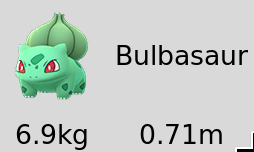
\includegraphics[width=12cm]{ressources/carte.png}
\captionof{figure}{Cartes mélangées}
\label{pique}
\end{center}
\begin{activite}
\begin{enumerate}
    \item Prendre le paquet de cartes mélangées et les étaler sur la table.
    \item Trier les cartes.
    \item Formaliser la méthode sous forme d'un algorithme.
\end{enumerate}
\end{activite}
\section{Transposer au tri de données}
\begin{activite}
\begin{enumerate}
    \item Implémenter 
\end{enumerate}
\end{activite}
\end{document}